\documentclass[]{article}
\usepackage{lmodern}
\usepackage{amssymb,amsmath}
\usepackage{ifxetex,ifluatex}
\usepackage{fixltx2e} % provides \textsubscript
\ifnum 0\ifxetex 1\fi\ifluatex 1\fi=0 % if pdftex
  \usepackage[T1]{fontenc}
  \usepackage[utf8]{inputenc}
\else % if luatex or xelatex
  \ifxetex
    \usepackage{mathspec}
  \else
    \usepackage{fontspec}
  \fi
  \defaultfontfeatures{Ligatures=TeX,Scale=MatchLowercase}
\fi
% use upquote if available, for straight quotes in verbatim environments
\IfFileExists{upquote.sty}{\usepackage{upquote}}{}
% use microtype if available
\IfFileExists{microtype.sty}{%
\usepackage{microtype}
\UseMicrotypeSet[protrusion]{basicmath} % disable protrusion for tt fonts
}{}
\usepackage[margin=1in]{geometry}
\usepackage{hyperref}
\hypersetup{unicode=true,
            pdftitle={MEGAHAND},
            pdfauthor={Ryan, John, Noah, Joe},
            pdfborder={0 0 0},
            breaklinks=true}
\urlstyle{same}  % don't use monospace font for urls
\usepackage{color}
\usepackage{fancyvrb}
\newcommand{\VerbBar}{|}
\newcommand{\VERB}{\Verb[commandchars=\\\{\}]}
\DefineVerbatimEnvironment{Highlighting}{Verbatim}{commandchars=\\\{\}}
% Add ',fontsize=\small' for more characters per line
\usepackage{framed}
\definecolor{shadecolor}{RGB}{248,248,248}
\newenvironment{Shaded}{\begin{snugshade}}{\end{snugshade}}
\newcommand{\KeywordTok}[1]{\textcolor[rgb]{0.13,0.29,0.53}{\textbf{#1}}}
\newcommand{\DataTypeTok}[1]{\textcolor[rgb]{0.13,0.29,0.53}{#1}}
\newcommand{\DecValTok}[1]{\textcolor[rgb]{0.00,0.00,0.81}{#1}}
\newcommand{\BaseNTok}[1]{\textcolor[rgb]{0.00,0.00,0.81}{#1}}
\newcommand{\FloatTok}[1]{\textcolor[rgb]{0.00,0.00,0.81}{#1}}
\newcommand{\ConstantTok}[1]{\textcolor[rgb]{0.00,0.00,0.00}{#1}}
\newcommand{\CharTok}[1]{\textcolor[rgb]{0.31,0.60,0.02}{#1}}
\newcommand{\SpecialCharTok}[1]{\textcolor[rgb]{0.00,0.00,0.00}{#1}}
\newcommand{\StringTok}[1]{\textcolor[rgb]{0.31,0.60,0.02}{#1}}
\newcommand{\VerbatimStringTok}[1]{\textcolor[rgb]{0.31,0.60,0.02}{#1}}
\newcommand{\SpecialStringTok}[1]{\textcolor[rgb]{0.31,0.60,0.02}{#1}}
\newcommand{\ImportTok}[1]{#1}
\newcommand{\CommentTok}[1]{\textcolor[rgb]{0.56,0.35,0.01}{\textit{#1}}}
\newcommand{\DocumentationTok}[1]{\textcolor[rgb]{0.56,0.35,0.01}{\textbf{\textit{#1}}}}
\newcommand{\AnnotationTok}[1]{\textcolor[rgb]{0.56,0.35,0.01}{\textbf{\textit{#1}}}}
\newcommand{\CommentVarTok}[1]{\textcolor[rgb]{0.56,0.35,0.01}{\textbf{\textit{#1}}}}
\newcommand{\OtherTok}[1]{\textcolor[rgb]{0.56,0.35,0.01}{#1}}
\newcommand{\FunctionTok}[1]{\textcolor[rgb]{0.00,0.00,0.00}{#1}}
\newcommand{\VariableTok}[1]{\textcolor[rgb]{0.00,0.00,0.00}{#1}}
\newcommand{\ControlFlowTok}[1]{\textcolor[rgb]{0.13,0.29,0.53}{\textbf{#1}}}
\newcommand{\OperatorTok}[1]{\textcolor[rgb]{0.81,0.36,0.00}{\textbf{#1}}}
\newcommand{\BuiltInTok}[1]{#1}
\newcommand{\ExtensionTok}[1]{#1}
\newcommand{\PreprocessorTok}[1]{\textcolor[rgb]{0.56,0.35,0.01}{\textit{#1}}}
\newcommand{\AttributeTok}[1]{\textcolor[rgb]{0.77,0.63,0.00}{#1}}
\newcommand{\RegionMarkerTok}[1]{#1}
\newcommand{\InformationTok}[1]{\textcolor[rgb]{0.56,0.35,0.01}{\textbf{\textit{#1}}}}
\newcommand{\WarningTok}[1]{\textcolor[rgb]{0.56,0.35,0.01}{\textbf{\textit{#1}}}}
\newcommand{\AlertTok}[1]{\textcolor[rgb]{0.94,0.16,0.16}{#1}}
\newcommand{\ErrorTok}[1]{\textcolor[rgb]{0.64,0.00,0.00}{\textbf{#1}}}
\newcommand{\NormalTok}[1]{#1}
\usepackage{longtable,booktabs}
\usepackage{graphicx,grffile}
\makeatletter
\def\maxwidth{\ifdim\Gin@nat@width>\linewidth\linewidth\else\Gin@nat@width\fi}
\def\maxheight{\ifdim\Gin@nat@height>\textheight\textheight\else\Gin@nat@height\fi}
\makeatother
% Scale images if necessary, so that they will not overflow the page
% margins by default, and it is still possible to overwrite the defaults
% using explicit options in \includegraphics[width, height, ...]{}
\setkeys{Gin}{width=\maxwidth,height=\maxheight,keepaspectratio}
\IfFileExists{parskip.sty}{%
\usepackage{parskip}
}{% else
\setlength{\parindent}{0pt}
\setlength{\parskip}{6pt plus 2pt minus 1pt}
}
\setlength{\emergencystretch}{3em}  % prevent overfull lines
\providecommand{\tightlist}{%
  \setlength{\itemsep}{0pt}\setlength{\parskip}{0pt}}
\setcounter{secnumdepth}{0}
% Redefines (sub)paragraphs to behave more like sections
\ifx\paragraph\undefined\else
\let\oldparagraph\paragraph
\renewcommand{\paragraph}[1]{\oldparagraph{#1}\mbox{}}
\fi
\ifx\subparagraph\undefined\else
\let\oldsubparagraph\subparagraph
\renewcommand{\subparagraph}[1]{\oldsubparagraph{#1}\mbox{}}
\fi

%%% Use protect on footnotes to avoid problems with footnotes in titles
\let\rmarkdownfootnote\footnote%
\def\footnote{\protect\rmarkdownfootnote}

%%% Change title format to be more compact
\usepackage{titling}

% Create subtitle command for use in maketitle
\newcommand{\subtitle}[1]{
  \posttitle{
    \begin{center}\large#1\end{center}
    }
}

\setlength{\droptitle}{-2em}

  \title{MEGAHAND}
    \pretitle{\vspace{\droptitle}\centering\huge}
  \posttitle{\par}
    \author{Ryan, John, Noah, Joe}
    \preauthor{\centering\large\emph}
  \postauthor{\par}
      \predate{\centering\large\emph}
  \postdate{\par}
    \date{11/8/2018}


\begin{document}
\maketitle

\subsection{R packages}\label{r-packages}

Tidyverse is a meta-package (a pack of packages) that is very commonly
used in R, and then Tensorflow and Keras are used for Machine Learning.
According to Martin, Keras was developed for Python, and then the same
dev developed it for R, so it is a framework that can be used in both
languages. That being said, we opted for scikit-learn.

\begin{Shaded}
\begin{Highlighting}[]
\CommentTok{# install.packages("tidyverse")}
\CommentTok{# install.packages("tensorflow", dependencies = TRUE)}
\CommentTok{# install.packages("keras", dependencies = TRUE)}

\KeywordTok{library}\NormalTok{(tidyverse)}
\end{Highlighting}
\end{Shaded}

\begin{verbatim}
## -- Attaching packages ----------------------------------------------------------------- tidyverse 1.2.1 --
\end{verbatim}

\begin{verbatim}
## v ggplot2 3.0.0     v purrr   0.2.5
## v tibble  1.4.2     v dplyr   0.7.6
## v tidyr   0.8.1     v stringr 1.3.1
## v readr   1.1.1     v forcats 0.3.0
\end{verbatim}

\begin{verbatim}
## -- Conflicts -------------------------------------------------------------------- tidyverse_conflicts() --
## x dplyr::filter() masks stats::filter()
## x dplyr::lag()    masks stats::lag()
\end{verbatim}

\begin{Shaded}
\begin{Highlighting}[]
\CommentTok{# library(tensorflow)}
\CommentTok{# library(keras)}
\end{Highlighting}
\end{Shaded}

\subsection{R package for interoperability with
Python}\label{r-package-for-interoperability-with-python}

This package includes functions that allow you to reference Python
objects in your R code, or source Python scripts from within R. I will
show an example of this shortly.

\begin{Shaded}
\begin{Highlighting}[]
\CommentTok{# install.packages("reticulate", dependencies = TRUE)}
\KeywordTok{library}\NormalTok{(reticulate)}
\end{Highlighting}
\end{Shaded}

\subsection{Reticulate}\label{reticulate}

With the reticulate package in R, Python code can be integrated into R
documents and used alongside R. This is especially convenient in the
RMarkdown document format for several reasons:

\begin{itemize}
\item
  R code and Python code can be called in discrete boxes, but within the
  same document
\item
  Objects built in either environment can be passed back and forth
  between languages
\item
  RMarkdown offers flexible export formats including pdf, slides, word,
  and html
\end{itemize}

This particular aspect of our project interested me due to the scale and
diversity of challenges in interoperability, both of which I have yet to
fully grasp.

\subsection{Python library imports, but in an RMarkdown
document}\label{python-library-imports-but-in-an-rmarkdown-document}

Frequently, the autocomplete available with Python functions and syntax
will work within a Python chunk in an RMarkdown document, but it is not
seamless yet. The words are, however, highlighted and colored as they
would be when working within a .py document (despite that not being the
case in this slidy presentation)

\begin{Shaded}
\begin{Highlighting}[]
\ImportTok{import}\NormalTok{ numpy }\ImportTok{as}\NormalTok{ np}
\ImportTok{import}\NormalTok{ pandas }\ImportTok{as}\NormalTok{ pd}
\ImportTok{import}\NormalTok{ matplotlib.pyplot }\ImportTok{as}\NormalTok{ plt}
\ImportTok{import}\NormalTok{ rpytools }\ImportTok{as}\NormalTok{ rpy}
\end{Highlighting}
\end{Shaded}

\subsection{Exploratory Data Analysis and
Visualization}\label{exploratory-data-analysis-and-visualization}

This is a Python script that grabs all of the ``.csv'' files in a
folder, and makes a list of the names. The script is saved as
``TrainingDataGrabber.py''

From the documentation for the glob() function:

The glob module finds all the pathnames matching a specified pattern
according to the rules used by the Unix shell, although results are
returned in arbitrary order. No tilde expansion is done, but *, ?, and
character ranges expressed with {[}{]} will be correctly matched. This
is done by using the os.scandir() and fnmatch.fnmatch() functions in
concert, and not by actually invoking a subshell. Note that unlike
fnmatch.fnmatch(), glob treats filenames beginning with a dot (.) as
special cases. (For tilde and shell variable expansion, use
os.path.expanduser() and os.path.expandvars().)

\begin{Shaded}
\begin{Highlighting}[]
\ImportTok{import}\NormalTok{ os}
\ImportTok{import}\NormalTok{ glob}
\NormalTok{path }\OperatorTok{=} \StringTok{'c:}\CharTok{\textbackslash{}\textbackslash{}}\StringTok{'}
\NormalTok{extension }\OperatorTok{=} \StringTok{'csv'}
\NormalTok{os.chdir(path}\OperatorTok{=} \StringTok{"C:/Users/joeje/Desktop/Academics/FAES/Intro_to_Python/MEGAHAND/TrainingData"}\NormalTok{)}
\NormalTok{Training_Data_Files }\OperatorTok{=}\NormalTok{ [i }\ControlFlowTok{for}\NormalTok{ i }\KeywordTok{in}\NormalTok{ glob.glob(}\StringTok{'*.}\SpecialCharTok{\{\}}\StringTok{'}\NormalTok{.}\BuiltInTok{format}\NormalTok{(extension))]}
\BuiltInTok{print}\NormalTok{(Training_Data_Files)}
\end{Highlighting}
\end{Shaded}

\subsection{Using Reticulate to source a Python
Script}\label{using-reticulate-to-source-a-python-script}

Here, I used R to source the Python script, create a list object
containing all of the file names in the ``TrainingData'' folder, and
then coerced an R DataFrame from that Python list for display.

\begin{Shaded}
\begin{Highlighting}[]
\NormalTok{reticulate}\OperatorTok{::}\KeywordTok{source_python}\NormalTok{(}\StringTok{"TrainingDataGrabber.py"}\NormalTok{)}

\NormalTok{Training_Data_Files}
\end{Highlighting}
\end{Shaded}

\begin{verbatim}
##  [1] "Chuck Grip.csv"     "Fine Pinch.csv"     "H. Open.csv"       
##  [4] "Hook Grip.csv"      "Key Grip.csv"       "No Move.csv"       
##  [7] "Power Grip.csv"     "Thumb Enclosed.csv" "Tool Grip.csv"     
## [10] "W. Abduction.csv"   "W. Adduction.csv"   "W. Extension.csv"  
## [13] "W. Flexion.csv"     "W. Pronation.csv"   "W. Supination.csv"
\end{verbatim}

\begin{Shaded}
\begin{Highlighting}[]
\NormalTok{knitr}\OperatorTok{::}\KeywordTok{kable}\NormalTok{(}\KeywordTok{as.data.frame}\NormalTok{(Training_Data_Files))}
\end{Highlighting}
\end{Shaded}

\begin{longtable}[]{@{}l@{}}
\toprule
Training\_Data\_Files\tabularnewline
\midrule
\endhead
Chuck Grip.csv\tabularnewline
Fine Pinch.csv\tabularnewline
H. Open.csv\tabularnewline
Hook Grip.csv\tabularnewline
Key Grip.csv\tabularnewline
No Move.csv\tabularnewline
Power Grip.csv\tabularnewline
Thumb Enclosed.csv\tabularnewline
Tool Grip.csv\tabularnewline
W. Abduction.csv\tabularnewline
W. Adduction.csv\tabularnewline
W. Extension.csv\tabularnewline
W. Flexion.csv\tabularnewline
W. Pronation.csv\tabularnewline
W. Supination.csv\tabularnewline
\bottomrule
\end{longtable}

\subsection{Using R for data tidying and
visualization}\label{using-r-for-data-tidying-and-visualization}

Next, I used the purrr package from R to apply a function I made in R
that tidys the data (removing extraneous columns and formatting) and
then creates a pre-set visualization for all of the files from the list
(that was made in Python.)

\begin{Shaded}
\begin{Highlighting}[]
\KeywordTok{source}\NormalTok{(}\StringTok{"C:/Users/joeje/Desktop/Academics/FAES/Intro_to_Python/MEGAHAND/Megamunge_Jitter.R"}\NormalTok{)}
\KeywordTok{library}\NormalTok{(purrr)}
\KeywordTok{setwd}\NormalTok{(}\StringTok{'TrainingData'}\NormalTok{)}
\KeywordTok{map}\NormalTok{(Training_Data_Files, Megamunge)}
\end{Highlighting}
\end{Shaded}

\begin{verbatim}
## [[1]]
\end{verbatim}

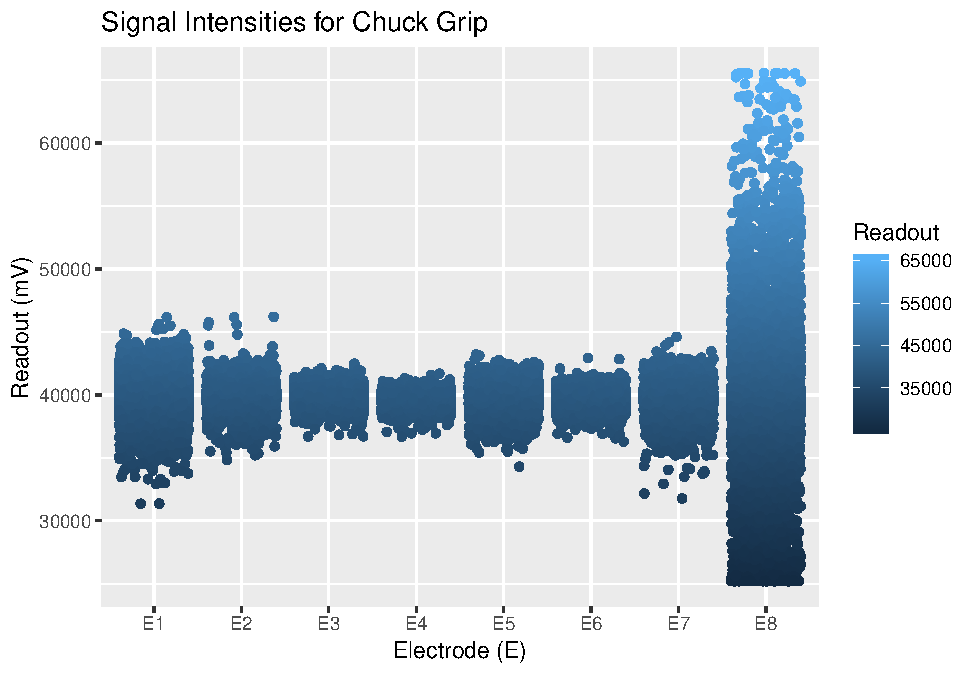
\includegraphics{Megahand_files/figure-latex/unnamed-chunk-6-1.pdf}

\begin{verbatim}
## 
## [[2]]
\end{verbatim}

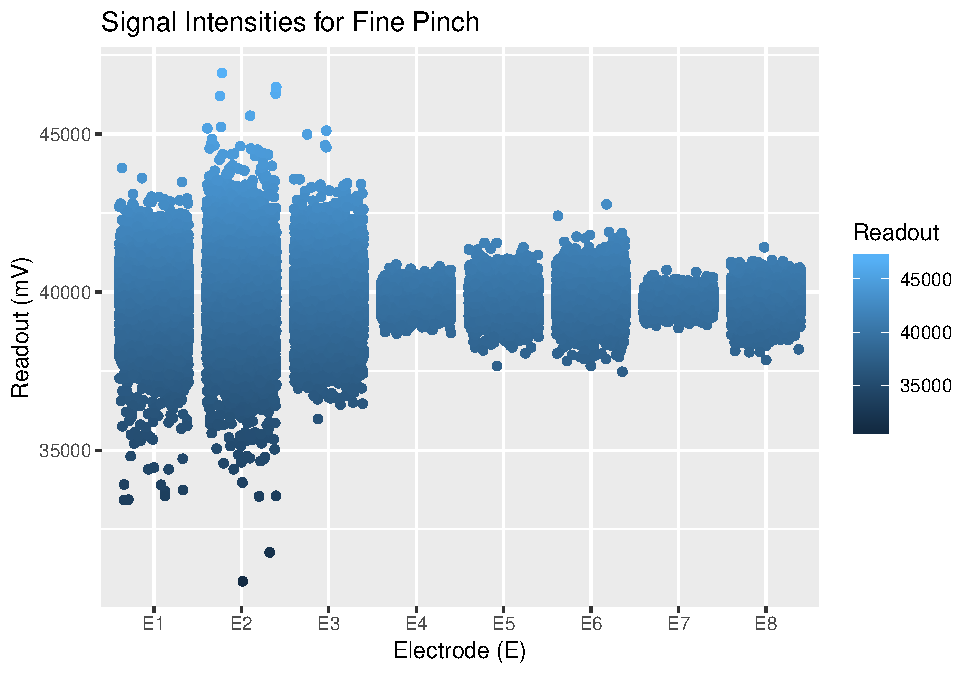
\includegraphics{Megahand_files/figure-latex/unnamed-chunk-6-2.pdf}

\begin{verbatim}
## 
## [[3]]
\end{verbatim}

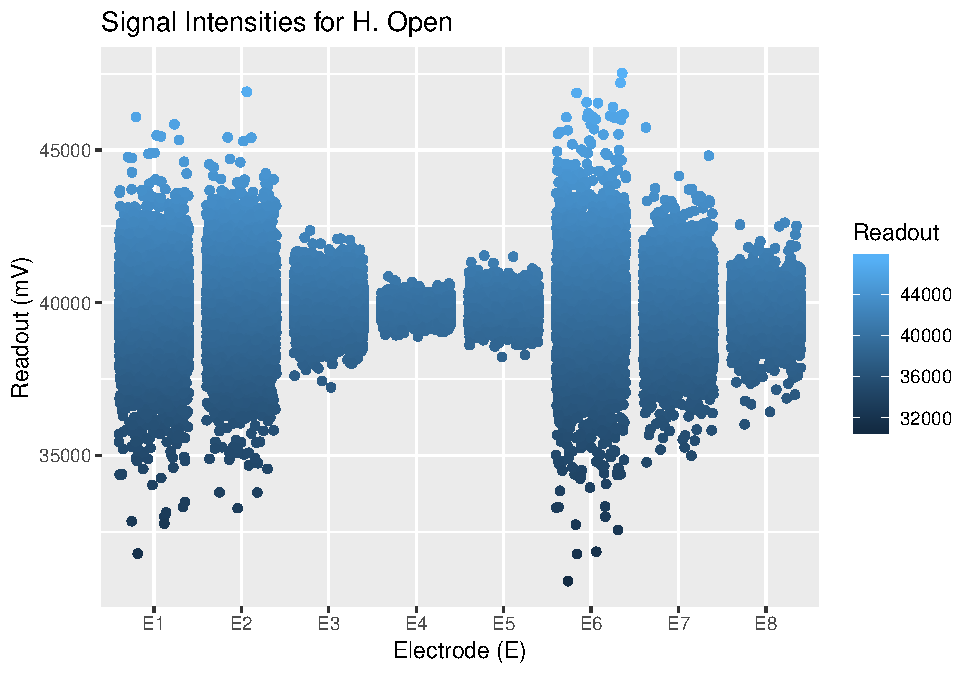
\includegraphics{Megahand_files/figure-latex/unnamed-chunk-6-3.pdf}

\begin{verbatim}
## 
## [[4]]
\end{verbatim}

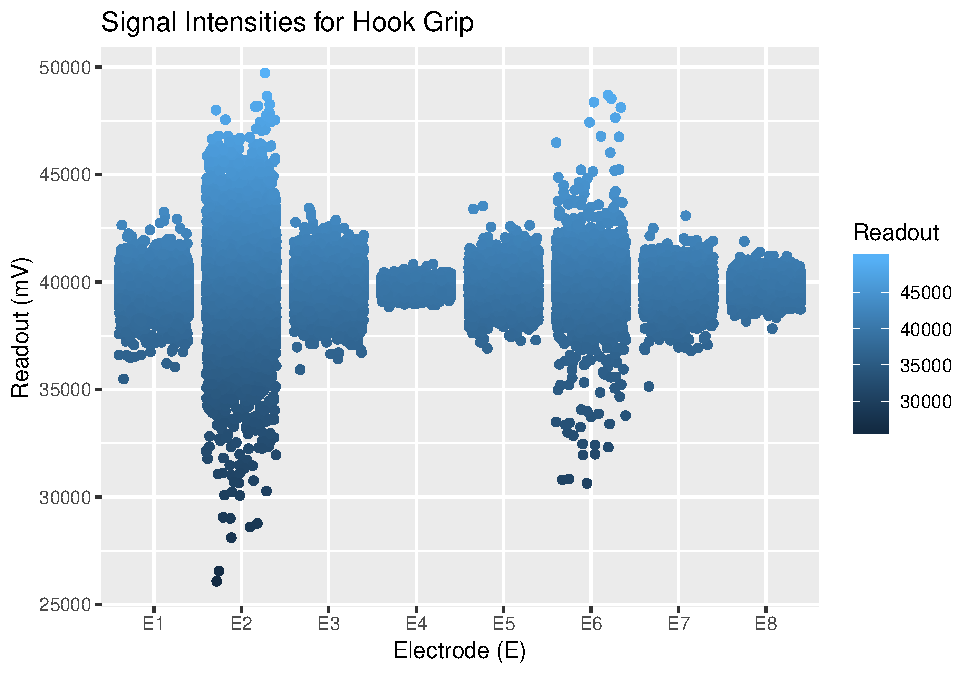
\includegraphics{Megahand_files/figure-latex/unnamed-chunk-6-4.pdf}

\begin{verbatim}
## 
## [[5]]
\end{verbatim}

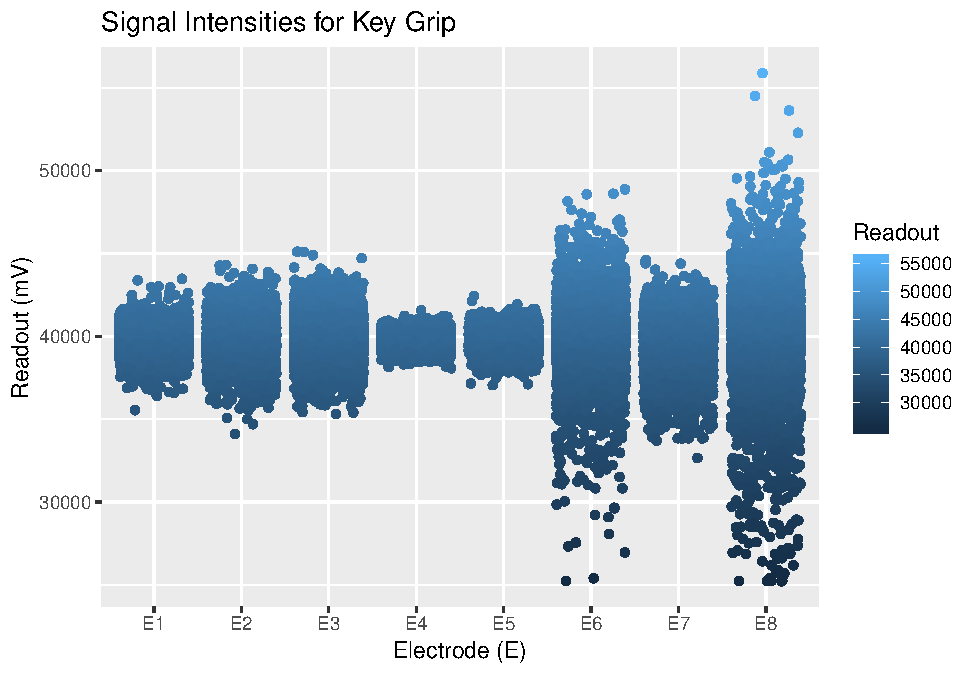
\includegraphics{Megahand_files/figure-latex/unnamed-chunk-6-5.pdf}

\begin{verbatim}
## 
## [[6]]
\end{verbatim}

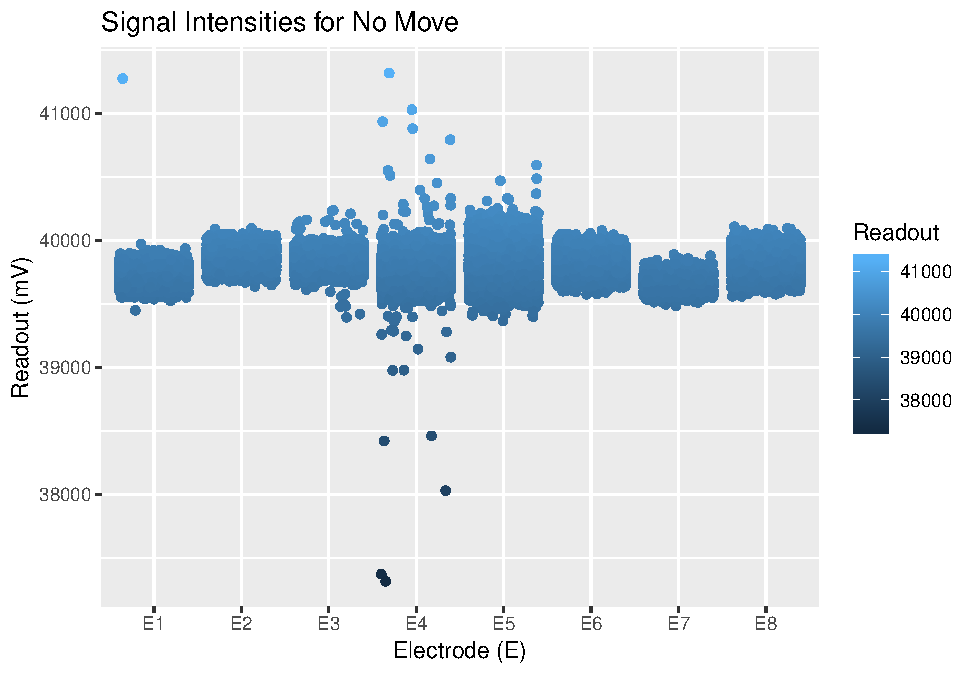
\includegraphics{Megahand_files/figure-latex/unnamed-chunk-6-6.pdf}

\begin{verbatim}
## 
## [[7]]
\end{verbatim}

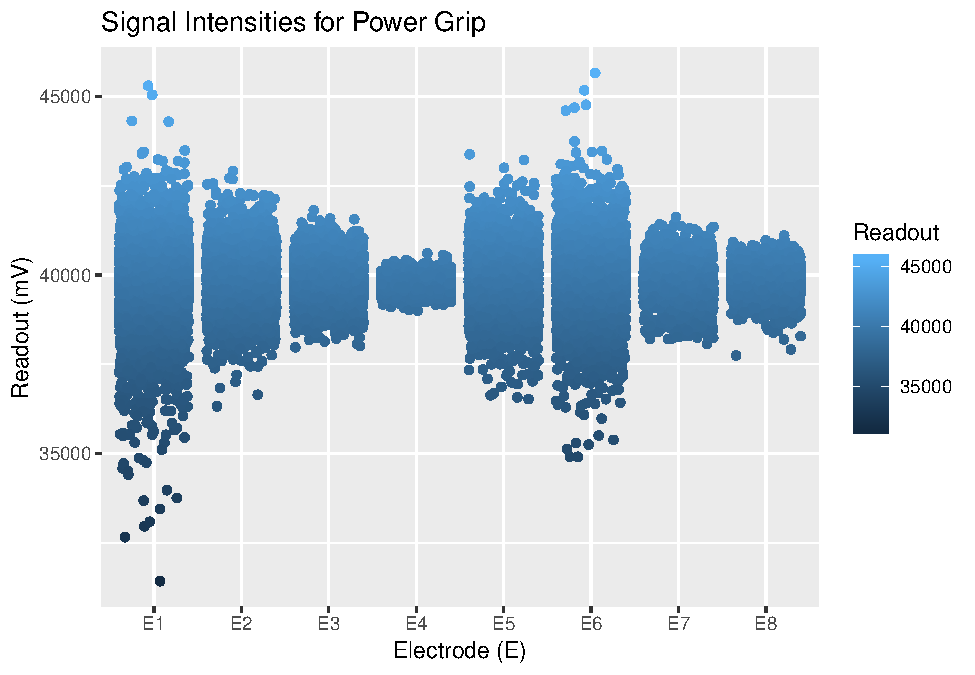
\includegraphics{Megahand_files/figure-latex/unnamed-chunk-6-7.pdf}

\begin{verbatim}
## 
## [[8]]
\end{verbatim}

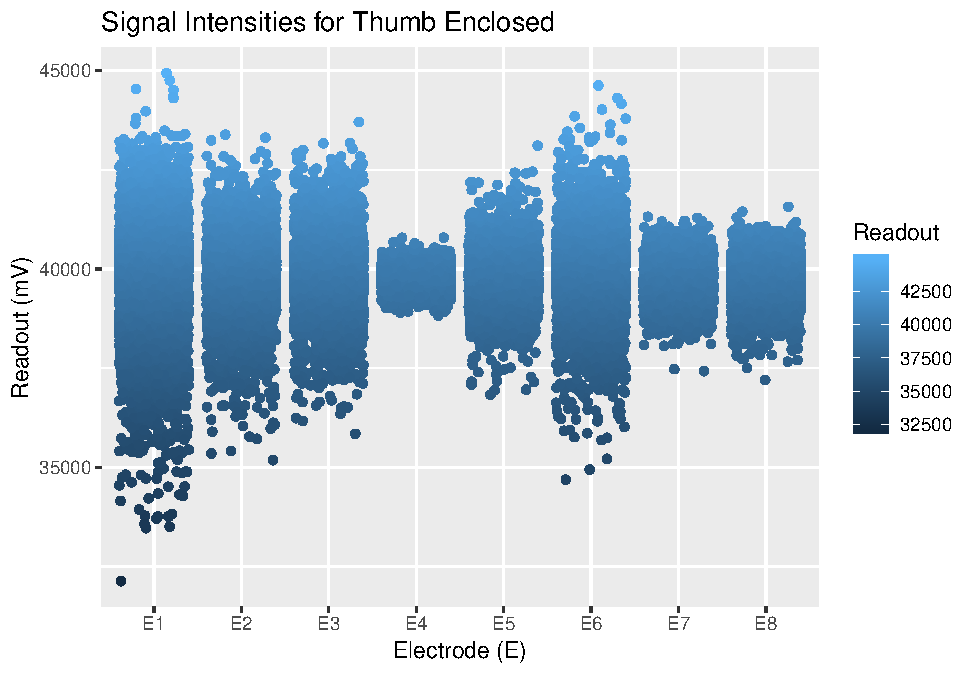
\includegraphics{Megahand_files/figure-latex/unnamed-chunk-6-8.pdf}

\begin{verbatim}
## 
## [[9]]
\end{verbatim}

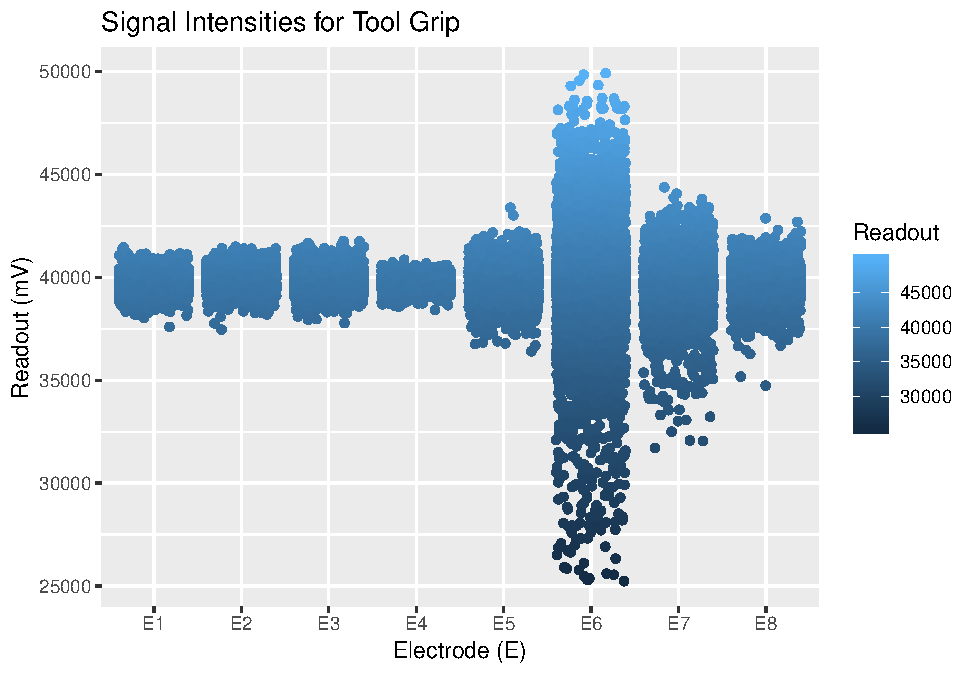
\includegraphics{Megahand_files/figure-latex/unnamed-chunk-6-9.pdf}

\begin{verbatim}
## 
## [[10]]
\end{verbatim}

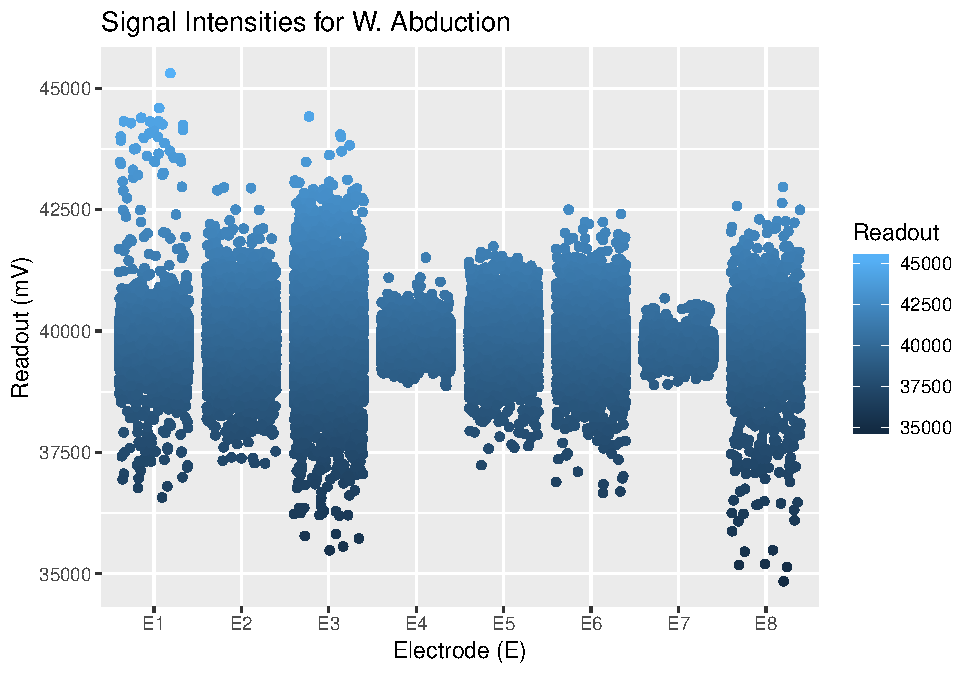
\includegraphics{Megahand_files/figure-latex/unnamed-chunk-6-10.pdf}

\begin{verbatim}
## 
## [[11]]
\end{verbatim}

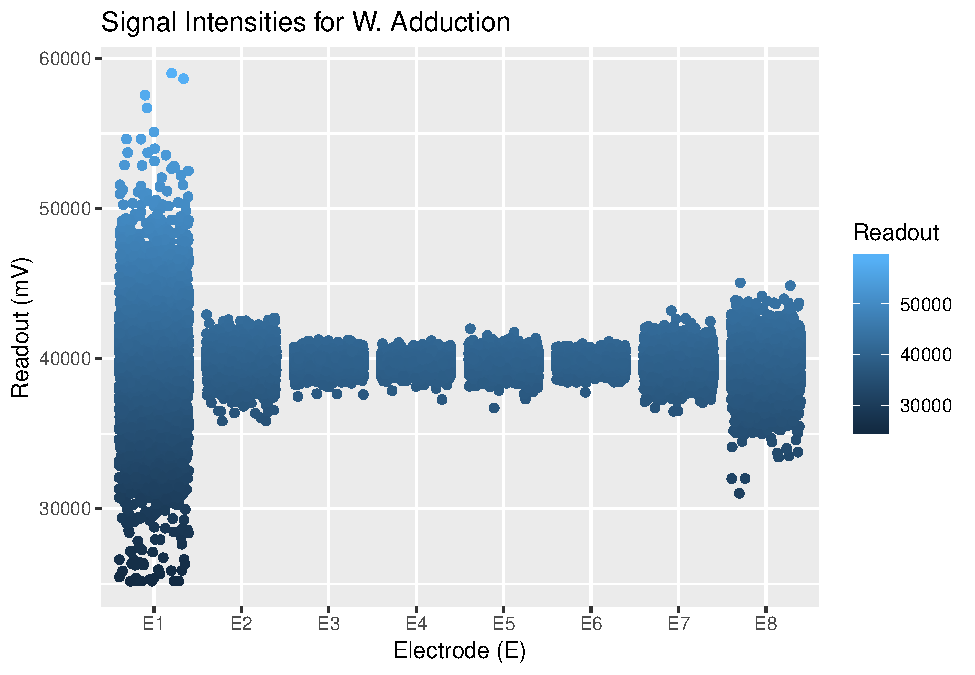
\includegraphics{Megahand_files/figure-latex/unnamed-chunk-6-11.pdf}

\begin{verbatim}
## 
## [[12]]
\end{verbatim}

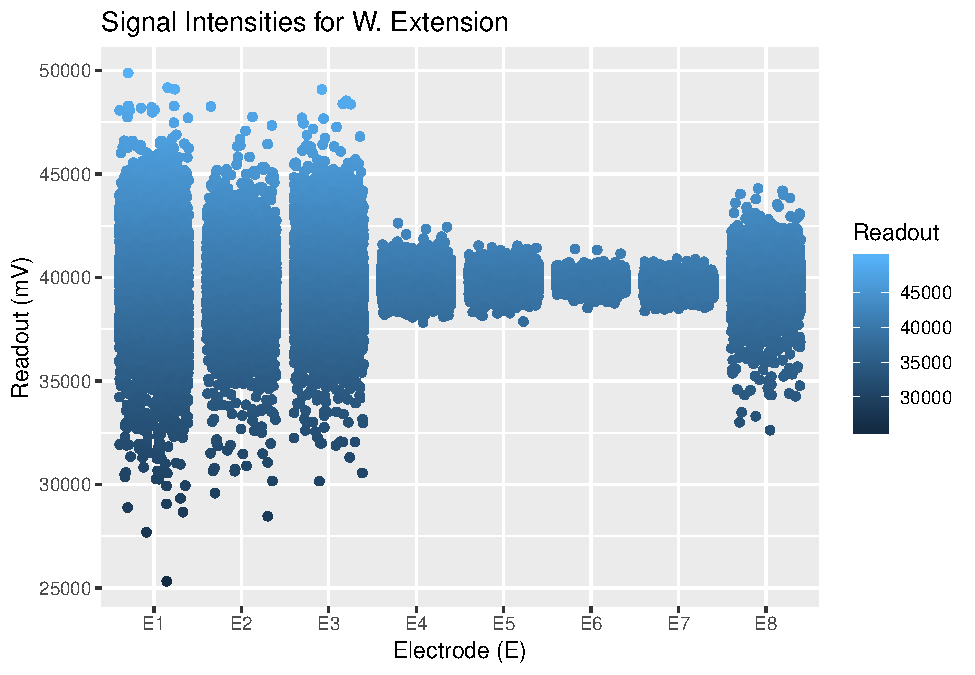
\includegraphics{Megahand_files/figure-latex/unnamed-chunk-6-12.pdf}

\begin{verbatim}
## 
## [[13]]
\end{verbatim}

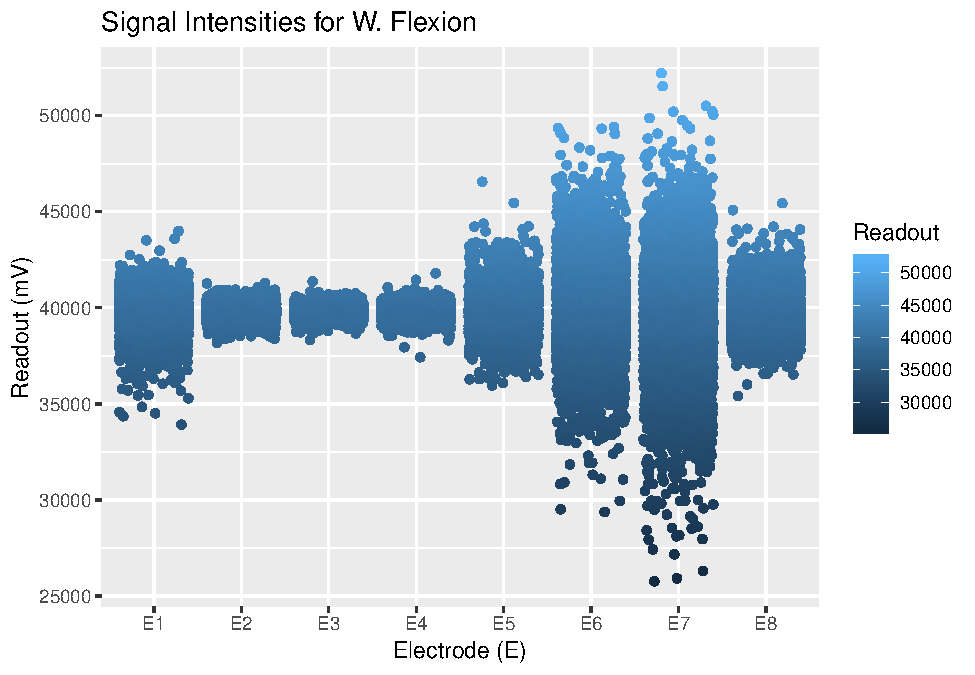
\includegraphics{Megahand_files/figure-latex/unnamed-chunk-6-13.pdf}

\begin{verbatim}
## 
## [[14]]
\end{verbatim}

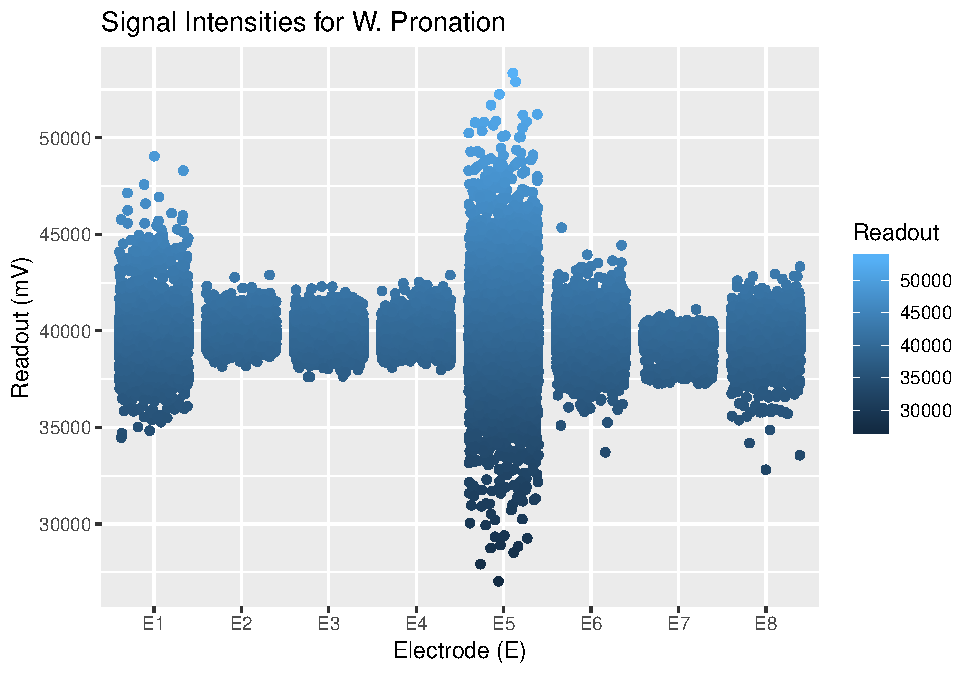
\includegraphics{Megahand_files/figure-latex/unnamed-chunk-6-14.pdf}

\begin{verbatim}
## 
## [[15]]
\end{verbatim}

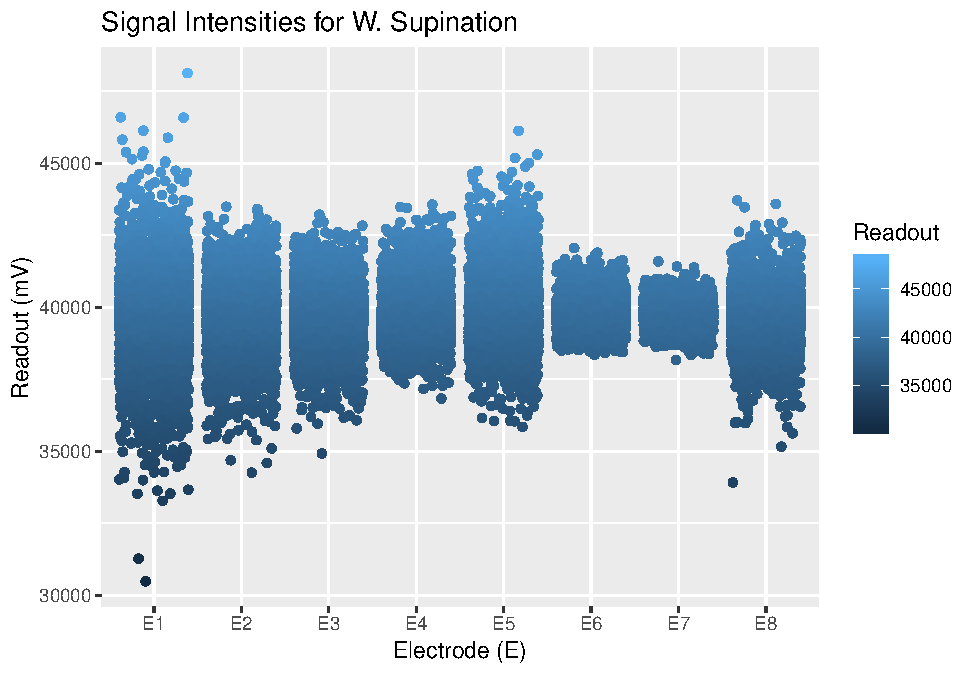
\includegraphics{Megahand_files/figure-latex/unnamed-chunk-6-15.pdf}


\end{document}
